\documentclass[11pt]{report}
\usepackage{graphicx}
\usepackage[a4paper, portrait, margin=1.6cm]{geometry}
\usepackage{enumitem}
\usepackage[hidelinks]{hyperref}
\newcommand{\ts}{\textsuperscript}

\begin{document}
\pagenumbering{gobble}
\hspace*{-\parindent}\hspace{-1em}
\begin{tabular}{p{3.8cm} p{13cm}}
    \vspace{0pt} 
    {%
	\setlength{\fboxsep}{0pt}%
	\setlength{\fboxrule}{0.75pt}%
    \fbox{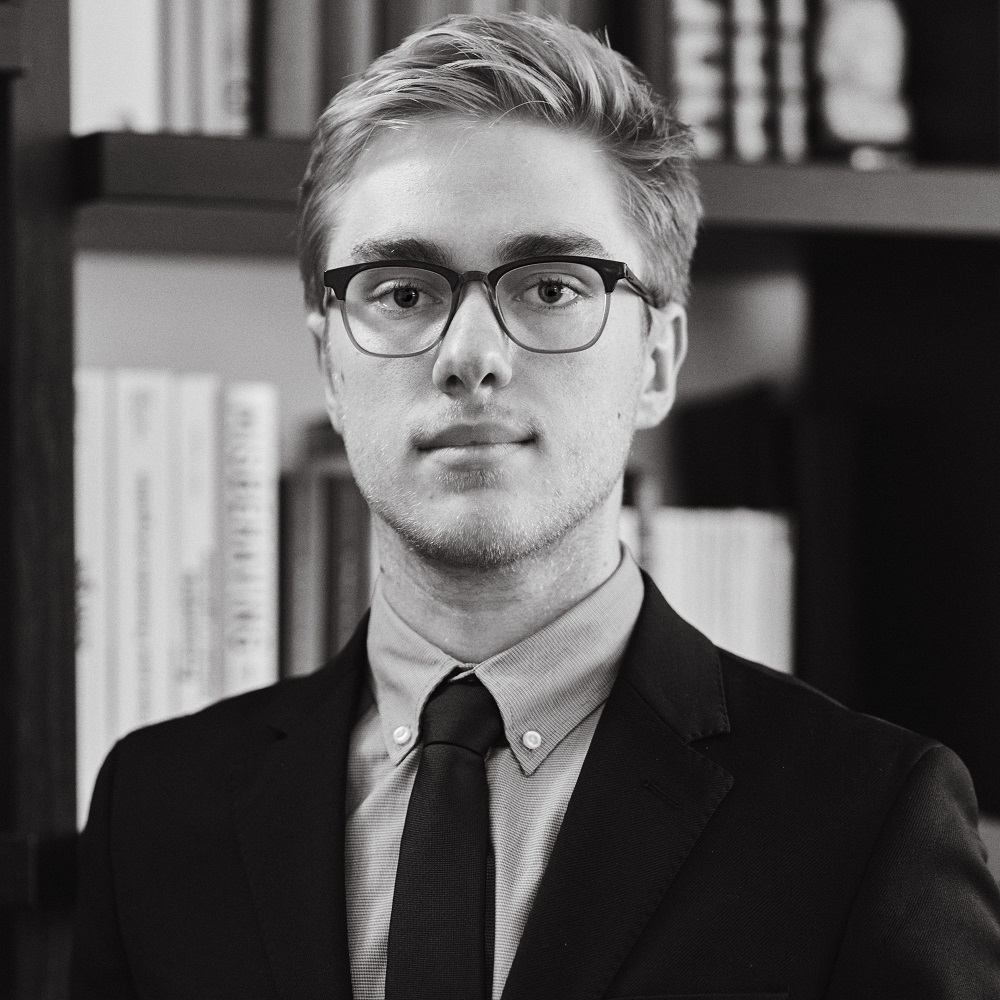
\includegraphics[scale=0.445]{picture.jpg}}%
    }%
    & 
    \vspace{0pt}
	\begin{Large}\textbf{PATRYK WISNIEWSKI}\end{Large}
	\newline \emph{Economics \& Statistics engineering student}
	\newline
	\newline Address: 155 Av. Pierre Brossolette, Montrouge, France
	\newline Email: \href{mailto:patryk@pwisniewski.com}{\underline{patryk@pwisniewski.com}}
	\newline Linkedin: \href{https://linkedin.com/in/pwisniewski02}{\underline{pwisniewski02}}
	\newline Téléphone: +33 6 95 30 31 18
	\newline Date de naissance: 18/07/2002
	\end{tabular}

	\begin{flushleft}
	\raisebox{-.6ex}{HIGHER EDUCATION} \hrulefill
	\end{flushleft}

	
\noindent\textbf{Master of Engineering \textbar\space Statistics,  Economics}
\hfill
\textbf{08/2023 - present} \\
\emph{ENSAE - Paris Polytechnic Institute}\\
Multidisciplinary engineering program combining a high-level of applied mathematics, economics, computer science, statistics, econometrics, and machine learning at the French National School of Statistics and Economic Administration, a leading institution in the fields of statistics, economics and data science.  \\

\noindent\textbf{Master 1 \textbar\space Quantitative Economics}
\hfill
\textbf{08/2022 - 05/2023} \\
\emph{Paris Dauphine University - PSL}\\
Program fully taught in English with advanced classes in micro, macro, game theory and econometrics  with additional teachings in data science. Master 1 project on the economics of privacy, focusing on the information asymmetries between data subjects and data platforms. \\
\\
\noindent\textbf{Bachelor \textbar\space Magistère, Economics}
\hfill
\textbf{09/2019 - 06/2022} \\
\emph{Pantheon Sorbonne \& Paris School of Economics}\\
Bachelor completed in the highly selective “Magistere of economics”, a program primarily focused on quantitative teachings with advanced math, stats and econometrics. Thesis on the stepping stone effect of short term contracts in the French labour market. 


	\begin{flushleft}
	\raisebox{-.6ex}{WORK EXPERIENCE} \hrulefill
	\end{flushleft}


\noindent\textbf{etiLab Mines Paris - PSL} \hfill Paris, France\\[0.1cm]
\textbf{Research assistant intern}\hfill \textbf{05/2023 - present} \\
Second internship at the centre of industrial economics in the etilab. I am currently working on the creation of clusters of medium size companies and the definition of their dynamics using machine learning techniques. I also work on a literature review about wage inequalities. \\[0.1cm]
\textbf{Research \& Data Intern}\hfill \textbf{06/2022 - 08/2022} \\
First internship at the centre of industrial economics in a newly created research program on mid-sized companies from the Paris region. During the internship, I assisted in the public data gathering, in the database
creation process and I was tasked to build an interactive web application for data visualisation.\\

\noindent\textbf{Narodowy Bank Polski} (Polish Central Bank) \hfill Warsaw, Poland\\[0.1cm]
\textbf{Research assistant intern}\hfill \textbf{05/2023 - present} \\
Short internship at the Polish Central Bank, during which I prepared a literature review on the monetary/fiscal policy-mix and the great inflation. I also worked on a VAR model trying to explain the strange occurrence of increases in delivery time with limited price hikes in some sectors. 


	\begin{flushleft}
	\raisebox{-.6ex}{SKILLS} \hrulefill
	\end{flushleft}



  \noindent\textbf{Programming Languages:}\hfill{Java / Python / R / SQL / Matlab} \\
  \textbf{Productivity:}\hfill LaTeX / Microsoft Office / Git\\
  \textbf{Web Technologies:}\hfill JavaScript / HTML5 / CSS / nodeJS / PHP  \\
  \textbf{Administration:} \hfill Windows (advanced) / GNU Linux (intermediate)\\
  \textbf{Languages:} \hfill French (native) / Polish (native) / English (C1 - TOEFL 106/120) 

	\begin{flushleft}
	\raisebox{-.6ex}{INTERESTS} \hrulefill
	\end{flushleft}

\noindent Analog \& Digital Photography / Electronics repair / Computer Hardware / Computer Networks  / Chess


\end{document}

